% #####################################################
% #####################################################
% #####################################################
\setchapterimage{figures/chap3/chapter_head_ICRF} % Optionally specify theheight
\setchapterpreamble[u]{\margintoc}
\chapter[High Power RF Devices for the Ion Cyclotron Range of Frequencies]{High Power RF Devices for the ICRF}
\label{chap:ICRF}

%\epigraph{On ne construit du solide que sur le passé. }{Thomas Stearns Eliot }
\epigraph{It's an experience like no other experience I can describe, the best thing that can happen to a scientist, realizing that something that has happened in his or her mind exactly corresponds to something that happens in nature. One is surprised that a construct of one's own mind can actually be realised in the honest-to-goodness world out there. A great shock, and a great, great joy.}{Leo Kadanoff}

%The purpose of RF engineering for plasma heating and current drive is to transmit several MW of RF power at frequencies, from the MHz to hundreds of GHz, and to deliver it into the plasma with the highest net efficiency as possible. The RF power is generated by one or few RF generators, then eventually combined and transported to the antennas. In order to optimize the global efficiency, it is desirable to have low loss, high electrical efficiency, low reflections, high reliability and actuators to adjust amplitude and phase. 

This chapter reviews the work done by the author on high power RF devices at CEA/IRFM for the Ion Cyclotron Range of Frequencies (ICRF). \marginnote{ICRF antennas being used mostly for Ion Cyclotron Resonance Heating plasma heating scheme, the terms ICRF and ICRH are seen are equivalent in this manuscript.} After introducing some generalities on ICRF systems in Section~\ref{sec:ICRH_antennas_general}, the Section~\ref{eq:WEST_ICRF_work} focuses on the work performed on the WEST ICRF antenna. Finally, the Section~\ref{sec:RF_contacts} reviews the results of the R\&D realized to develop electrical contacts compatible with high RF power in vacuum for the ITER ICRF antenna. 


% #####################################################
% #####################################################
% #####################################################
\section[Generalities]{Generalities on ICRF Antennas}\label{sec:ICRH_antennas_general}
\marginnote{Part of this section are taken from \citeauthyear{hillairet2020-1}.}

% #####################################################
% #####################################################
\subsection{Coupling Elements}
In order to excite the Fast-Waves in the Ion Cyclotron range of frequencies ($f=$30-80~MHz) as required for plasma heating, the wave electric field needs to be perpendicular to both $\Bbf_0$ and $\mathbf{k}$. In this range of frequencies, the wavelength of the electromagnetic waves is of order of few meters, so larger or of the same order as the machine size. To excite the Fast-Wave, ICRF antennas usually consist in array of loop radiators similar to strip-lines, or \textit{straps}, to excite waves directly inside the vacuum vessel (Figure~\ref{fig:icrhantennasimplified}). These straps are oriented perpendicularly to the direction of the magnetic field $B_0$\footnote{In tokamaks, the total magnetic field being slightly tilted with respect to the toroidal direction, straps should have a complex shape to produce fields with the proper polarization. While possible and more accessible nowadays than before with modern manufacturing techniques, building such straps is complex and most antennas use strap oriented in the poloidal direction, i.e. perpendicular to the toroidal magnetic field.}. The antenna geometry and the amplitude and phase distribution of the flowing RF currents $J_{RF}$ on these straps shapes the wavenumber spectrum $E_{RF}(k)$ excited by the antenna. The antenna having a characteristic toroidal size (of tens of centimetres) much smaller than the wave wavelength, most plane waves excited by the antenna are evanescent. The distance to the plasma is thus a crucial parameter for the coupling performances, so antennas are generally made conform as possible to the plasma to minimize the distance from the strap to the plasma. 

\begin{figure}
	\centering
	\includegraphics[width=0.9\linewidth]{figures/chap3/ICRH_antenna_simplified}
	\caption{Simplified schematic of a classic ICRF antenna in a tokamak.}
	\label{fig:icrhantennasimplified}
\end{figure}


%RDL\sidecite{owens1985}

% #####################################################
\subsection{Faraday Screen}
Unfortunately, it was identified early that coupling structures do not excite only Fast-Waves but also Slow-Waves \sidecite{evrard1982-1}. Slow-Waves are produced by RF currents parallel to the magnetic field as well by oscillating space charges on the antenna structure. For this reason, early ICRF experiments introduced the use of electrostatic shield, or \textit{Faraday Screen} \sidecite{england1989}. 

A Faraday Screen is formed by an array of metallic strips (or bars), aligned with the total magnetic field \sidecite{bures1990}. By screening the electric field components parallel to the strips/bars (Figure~\ref{fig:icrhfaradayscreenprinciple}), it aims acting as a polarizer, to filter out specifically the undesirable Slow-Wave. A denser screen better isolates the central conductor of the antenna from the plasma, but it also causes significant magnetic shielding and enhanced Ohmic losses in the screen \sidecite{faulconer1983}, leading to actively cooled structures. Various experiments have shown the benefits of Faraday Screen \sidecite{noterdaeme1986, bures1990, myra1990}, but some also concluded that heating performance of unshielded antenna was similar to that of a shielded antenna \sidecite{nieuwenhove1991, nieuwenhove1992}.  Although it might be necessary to keep a Faraday shield for other reasons, such as decoupling thermal and mechanical stresses on plasma facing components, the question of the necessity of a Faraday Screen in future ICRF antennas is still an open question in the ICRF community \sidecite{noterdaeme2019}. 

\begin{marginfigure}
	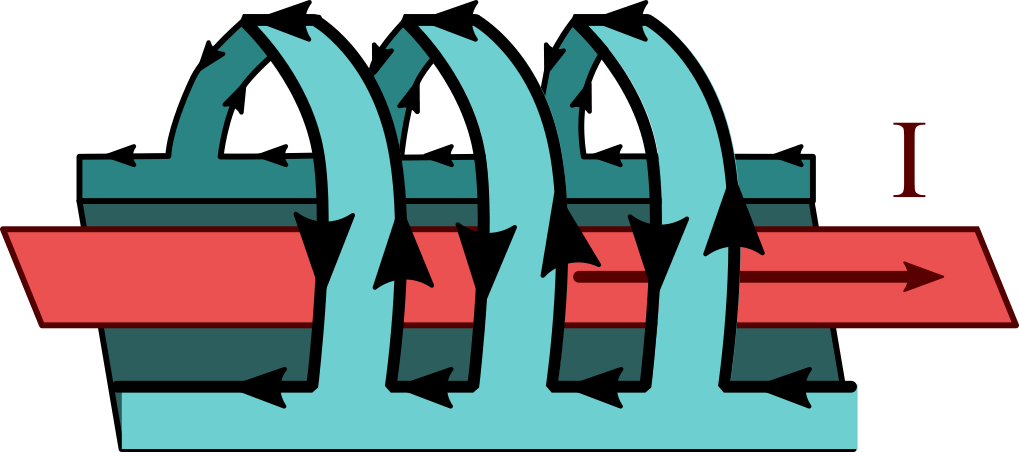
\includegraphics[width=1.0\linewidth]{figures/chap3/WEST_ICRH/ICRH_Faraday_Screen_Principle}
	\caption{Surface current induced on a shield above a perfectly conducting plane by the enclosed line current $I$. Surface currents shown is superposition of currents on inner and outer blade faces.}
	\label{fig:icrhfaradayscreenprinciple}
\end{marginfigure}

% #####################################################
\subsection{Matching}\label{sec:ICRH_matching_systems}
From the RF engineer point of view, an ICRF system is equivalent to a transmission line loaded with a complex impedance (Figure~\ref{fig:icrhantennacircuitmodel}). The antenna can be viewed as an impedance whose properties depend on the plasma. 

\begin{figure}[h]
	\centering
	\includegraphics[width=0.9\linewidth]{figures/chap3/ICRH_antenna_circuit_model}
	\caption{Simplified model of a ICRF system.}
	\label{fig:icrhantennacircuitmodel}
\end{figure}

A single strap element can be modelled by a line terminated with a lumped impedance $Z_L = R + j X$ \sidecite{bhatnagar1982}. Without plasma, the resistive part of this load represents the antenna Ohmic losses, which are generally small ($R \propto 10^{-1}~\si{\Omega}$). In front of a magnetized plasma, part of the waves are coupled to the plasma and the resistive part of the load increases. Hence, for the circuit point of view, coupling is indistinguishable from increasing losses. In most tokamak experiments, the resistive loading is in the 0.5 to 10 $\si{\Omega}$ range \sidecite{pinsker1998}. The reactive part is mostly inductive. Its value depends mainly on the strap and antenna geometry and is generally much higher than the resistive part. In addition, changes of the resistive part are also correlated with changes in the reactive part \sidecite{pinsker1998}\sidenote{The electrical equivalent length of the antenna is then usually reduced when facing a plasma.}. Since the characteristic impedance of the transmission line $Z_0$ is usually between 30 to 50~$\si{\Omega}$, we always have $R \ll Z_0$ and hence a matching unit is necessary to maximize the power coupled to the plasma by the antenna.

Moreover, sudden changes in antenna loading arise in tokamaks operating in H-mode. During plasma perturbations (such like ELMs), loading rises on a time scale of around 100\si{\micro s} and subsequently decays on a time scale of a few milliseconds. This sub-millisecond timescale represents a challenge to any dynamic impedance matching scheme implemented in ICRF systems\sidecite{hofmeister1994, ladurelle1997, evrard2005, noterdaeme2005, prechtl2009, grine2012, lin2015}, because their response time is not fast enough. To cope with these fast events, inherently load insensitive schemes, or \textit{load-resilient}, are desirable. At ASDEX-Upgrade, the load resilient system used to maintain the RF power during H-mode is exclusively the 3dB hybrid coupler system. The reflected power is mainly redirected toward a dummy load thanks to the symmetrical properties of the 3dB coupler. At JET, three different load resilient systems are employed. Firstly, a hybrid system feeds antennas A and B. Secondly, a conjugated-T system (resilient antenna) with internal matching is plugged to the ITER-Like Antenna (ILA). Part of the matching is made by vacuum capacitors connected close to the antenna. Thirdly, a conjugated T system with external matching feeds antennas C and D. Part of the matching is made by phase shifters connected far from the antennas.


\subsection{RF Sheaths}\label{sec:RF_sheaths}
Early ICRF experiments have reported non-linear interactions between high power RF waves and edge plasma, leading to the production of influx of impurities which prevented efficient heating of the plasma \sidecite{rothman1966}. Since then, despite improvements in antenna design and plasma operation which substantially reduced these undesirable phenomenon \sidecite{noterdaeme1993}, it still remains an important operational limitation of ICRF \sidecite{noterdaeme2019-1}. One mechanism leading to the release impurities during ICRF operation is RF sheaths rectification. 

Because of their mass difference, ions and electrons motions behave differently along magnetic field lines: electrons accumulate faster than ions on Plasma Facing Components (PFC) and form a thin negatively biased layer that repulses electrons and attracts ions. This attraction increases the  parallel energy of ions attracted into the wall and thus enhance the ion bombardment of the PFC. Ions impacting the PFC can cause sputtering of impurities that can reach and contaminate the plasma. In the presence RF waves parallel to the magnetic field lines (which corresponds to the Slow-Wave polarization) driven by ICRF antenna, sheaths are enhanced. Instead of being constant in time, DC potential drop across the sheath is then the superposition of a DC component and a RF oscillations, called \textit{RF-induced sheath rectification}. This  mechanism has been identified as a major reason for the increased interaction with the wall as is still an intense research topic \sidecite{colas2019, bobkov2019}.



\section{WEST ICRF Antenna}\label{eq:WEST_ICRF_work}

% #####################################################

\subsection{WEST ICRF Antennas Design}\label{eq:WEST_ICRH_antenna}
\marginnote{Parts of this section are taken from \citeauthyear{hillairet2015-2} and CEA/IRFM internal reports made in 2013-2014 during the design of the WEST ICRF antennas.}

\subsubsection{Context}
Three new identical ELM-resilient and CW power ICRF antennas have been designed for WEST. The ELM resilience property is obtained through an internal conjugate-T electrical scheme with series capacitors\sidecite{bosia2003-1}. The antenna design is based on a previously tested prototype in 2004 and 2007 at 48~MHz \sidecite{vulliez2008, argouarch2009}, illustrated in Figure~\ref{fig:proto2007antenna}. 

\begin{figure}[h]
	\centering
	\includegraphics[width=1.0\linewidth]{figures/chap3/WEST_ICRH/proto2007_antenna}
	\caption{CAD model of the "2007 Prototype" antenna.}
	\label{fig:proto2007antenna}
\end{figure}

In the frame of the Associated Laboratory in the fusion field between IRFM and ASIPP, the 2007 design has been upgraded for WEST in order to: 
\begin{itemize}
	\item improve the power capabilities and coupling resistance from the previous prototype \sidecite{helou2015-1}
	\item increase the nominal frequency range to 55~MHz to match WEST scenarios \sidecite{bourdelle2015}
	\item allow CW operation with actively cooled components \sidecite{chen2015, vulliez2015}.
\end{itemize} 

The 2013 panorama of worldwide ICRF system operational domains is illustrated in Figure~\ref{fig:westicrhcomparaisonothermachines}. The next ICRF system under realization is the one of ITER, which combines both high power and high durations. 

\begin{figure*}
	\centering
	\includegraphics[width=1.0\linewidth]{figures/chap3/WEST_ICRH/WEST_ICRH_comparaison_other_machines}
	\caption{2013 panorama of main ICRF system operational domains (independently of plasma conditions)}
	\label{fig:westicrhcomparaisonothermachines}
\end{figure*}

All the aspects previously listed led to iterate between RF and mechanical design, with generally opposite constraints and necessary compromises\sidenote{In order to improve the mechanical assembly of the WEST antenna in comparison to the 2007 prototype, the main dimensions changes have been proposed by K.Vulliez, A.Argouarch and P.Mollard for the conceptual design review in 2013 and assessed after from the RF point of view in an internal note \citeauthyear{hillairet2014-1}}. While the ICRF system upgrade for the WEST project also concerned the generator update and the moving of an antenna from port Q5 to port Q4A, this section only focuses on the antenna design. 


\begin{figure}
	\centering
	\includegraphics[width=0.7\linewidth]{figures/chap3/WEST_ICRH/proto2007_antenna_cut}
	\caption{Nomenclature of the ICRF 2007 or WEST antenna: The "Bridge" defines the antenna section which purpose is to split the input power toward both capacitors of half an antenna. The outer conductor of the coaxial input is connected to the antenna box while the inner conductor is connected to the bridge.}
	\label{fig:proto2007antennacut}
\end{figure}


% ###################################################
\subsubsection{Front Parts}
\begin{marginfigure}
	\centering
	\includegraphics[width=0.8\linewidth]{figures/chap3/WEST_ICRH/WEST_front_face_evolution1}
	\caption{Evolution of 2D CAD models for coupling optimization. This figure is similar to a cross-section of the geometry of the figure~\ref{fig:westfrontfaceevolution2}. }
	\label{fig:westfrontfaceevolution1}
\end{marginfigure}

Compared to the 2007 prototype, the front face of the WEST ICRF antennas have undergone few major changes in order to meet the following objectives:
\begin{enumerate}
	\item Increase the antenna overall coupling resistance $R_c$
	\item Increase the nominal antenna frequency to 55~MHz
	\item Water-cool the whole antenna, in particular the straps, the antenna box and the Faraday screen
	\item Minimize sheaths potential
\end{enumerate}

Increasing the coupling resistance allows coupling more power for a given set of voltages and currents. In other words, it also allows lowering capacitor voltages (and electric field) and currents for a given coupled power, which has operational and safety benefits\footnote{In addition, the capacitor manufacturer COMET has lowered the maximum voltage and current specifications on its products between 2004 and 2013.}. 

The frequency increase is a practical consequence of the changes of Tore Supra to become WEST: as the plasma volume was reduced and  shifted toward the high field side of the machine, locating the (hydrogen minority) cyclotron resonance in the plasma centre requires higher RF frequencies. The desired frequency band of the ICRF system for WEST was thus asked to be 48-60~MHz. RF plant has predefined frequencies centred around 48, 53, 55.5, 57 and 63~MHz $\pm$ 2~MHz.
 
\begin{marginfigure}
	\centering
	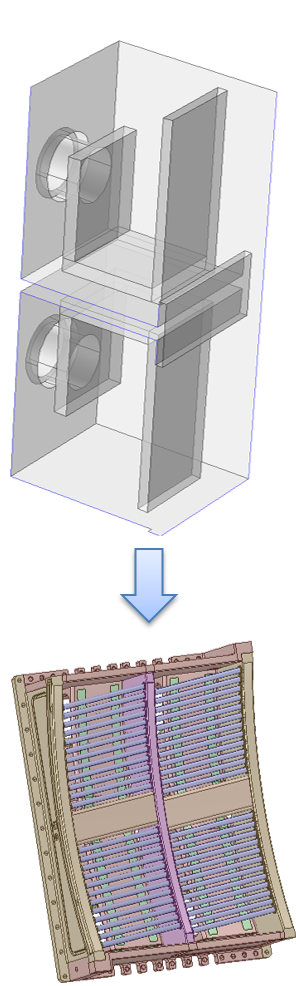
\includegraphics[width=0.8\linewidth]{figures/chap3/WEST_ICRH/WEST_front_face_evolution2}
	\caption{Evolution of 3D CAD models for coupling optimization.}
	\label{fig:westfrontfaceevolution2}
\end{marginfigure}

From July 2013 to May 2014, the coupling of various models have been assessed using the COMSOL finite element software. Perfectly Match Layers (PMLs) boundary conditions adapted to plasma fast wave were used in 2D and 3D\sidecite{jacquot2013, colas2019}. Starting from the 2007 prototype geometry, the effects of geometrical modifications on coupling resistance have been assessed, from very simplified parametrized 2D (Figure~\ref{fig:westfrontfaceevolution1}) to almost final 3D geometries (Figure~\ref{fig:westfrontfaceevolution2}). These models used first experimental density profiles obtained in Tore Supra in 2007 (pulse \#40574) before using assumptions of WEST density profiles. In this pulse, an L-mode plasma has been moved horizontally over 5 cm in front of the load-resilient antenna prototype to assess its coupling properties at 48 MHz. The calculations have been performed for 8 profiles in order to make relative comparisons of the coupling resistance. 2D model run in few minutes while 3D models typically required ten to twenty hours depending on their complexity and the distance to the cut-off density on a desktop computer. 

These parametrized models allowed us to assess the relevant geometrical parameters (strap thickness, width, and distances to the plasma cut-off and antenna box) affecting the coupling resistance. In order to optimize the coupling resistance in dipole configuration, the thickness of the strap has been kept as low as possible (between 13 and 15 mm) while ensuring sufficient stiffness, since they are water cooled through 70$\si{\degreeCelsius}$/30~bars inner channels. As an example, at 57~MHz, increasing the strap thickness by 15~mm decreased the coupling resistance by 25\% for the same plasma loading. The coupling resistance of the new antennas has been increased compared to the prototypes one in particular by reducing the distance between the strap and the Faraday screen bars from 52~mm to 34~mm and by supressing a vertical septum which was masking a portion of the straps in the prototype (Figure~\ref{fig:westfrontfaceevolution1}). 

Each antenna is equipped with four internal COMET tunable vacuum capacitors, with capacitances ranging from 15~pF to 150~pF and specifically upgraded for CW operation. In order to operate the antenna at a higher frequency (55~MHz vs the 48~MHz of the prototype) with the same capacitance range, the straps electrical length has been reduced in order to decrease their reactance $X_s$. However, increasing the coupling resistance also decreases the strap reactance $X_s$ {\sidecite{pinsker1998, helou2018}. Hence, trade-offs were unavoidable between coupling efficiency and impedance matching as the desired frequencies\footnote{Other trade-off have been made due to the following reasons. Bringing closer the strap and its feeder leads to reduce the coupling resistance (-23\% decrease of the coupling resistance for 50~mm distance reduction). Increasing the toroidal width of the straps led to reduce the strap reactance but also to decrease the coupling resistance (-50\% decrease of the coupling resistance for +40~mm width increase). It has been kept to 130~mm, the same value as for the prototype.}. 

As the design of the antenna progressed, the coupling of few milestone CAD 3D models has been calculated with the TOPICA code \sidecite{milanesio2009} with the same plasma scenarios to assess the impact of mechanical design evolutions on the coupling performances.

RF circuit optimizations have been first conducted on a single conjugate-T with uncoupled straps loaded with impedances. Thereafter, full-wave models of the T-junction, impedance transformer and vacuum feedthrough have been taken into account in ANSYS Designer®. This allows pushing realistic RF excitations into the full-wave ANSYS HFSS® model in order to deduce the heat flux topologies over the devices, which then can be easily imported in ANSYS Mechanical® for thermal modelling. Capacitors have been modelled using equivalent circuits. Finally, an electric circuit of the full antenna using TOPICA impedance matrices has been simulated. This model has been used to deduce the realistic capacitor sets, current and voltage values to be expected for various plasma scenarios. A full-wave modelling of the capacitor has also been performed and integrated into a RF circuit solver to confirm the approach.

Expected electron density profiles for WEST H-mode plasmas have also been used to load the antenna model. A set of profiles have been calculated for 3 different line average densities. Since the plasma volume in WEST is smaller than in Tore Supra, the antennas are located closer to the centre of the machine to keep the same gap from the antenna to the plasma. Three radial locations of the antenna have been used (R=3, 2.975 and 2.95 m) to model the coupling in TOPICA with these profiles, with the toroidal curvature of the plasma adjusted according to the WEST magnetic ripple. As no data were available for H-mode temperature profile, L-mode profile has been used. It has to be noted than the private plasma located between the antenna limiters has not been included in the TOPICA models.

Using the maximum capacitors currents and voltages (915 A and 54 kV peak respectively) the maximum coupled power has been calculated. In order to balance the top and bottom strap current magnitudes, one can allow the launchers input impedances to have an additional imaginary part. It might increase the VSWR but still allowing higher coupled power: an unbalanced current distribution can lead to currents/voltages exceeding the maximum limits at one strap while they are by far respecting the limits for the other one. %FIGURE1 illustrates the maximum coupled power achievable for the three antennas with respect to capacitors current and voltage limitations, for two matching strategies (VSWR=1:1 or VSWR<1.7:1). In this curve, the antennas have been matched for each coupling resistance point. 

%\todo{P vs Rc curve}



% ###################################################
\subsubsection{Rear Parts}
\begin{marginfigure}
	\centering
	\includegraphics[width=0.9\linewidth]{figures/chap3/WEST_ICRH/bridge_evolution}
	\caption{Modification of the bridge section from 2007 prototype (top) to WEST (bottom). The input transmission line has been made in-axis}
	\label{fig:bridgeevolution}
\end{marginfigure}

In order to reduce the manufacturing cost as well as to simplify the mechanical assembly design of the bridge, it has been proposed to design the bridge symmetrical with respect to its input transmission line. An idealized bridge/antenna box geometry which dimensions corresponding to the 2007 Prototype has been created and compared to one with an in-axis input transmission line (Figure~\ref{fig:bridgeevolution}). As minor changes were observed on both reflection and transmission, the WEST ICRF antenna bridges has been made symmetrical with respect to the input transmission line.

\begin{marginfigure}
	\centering
	\includegraphics[width=0.8\linewidth]{figures/chap3/WEST_ICRH/bridge_evolution2}
	\caption{Illustration of the bridge/antenna box inner dimensions $d_1$, $d_2$ and $d_3$.}
	\label{fig:bridgeevolution2}
\end{marginfigure}

Also in order to facilitate the mechanical assembly of the antenna, in particular the water pipes and diagnostic cables connection, it has been proposed to enlarge the distance between the rear part of the antenna box and the rear part of the bridge, ie. the dimensions $d_1$, $d_2$ and $d_3$ are illustrated in Figure~\ref{fig:bridgeevolution2}. The influence of each dimensions on RF performances have been assessed and it was proposed to keep the 2007 prototype ($d_1$=17.7~mm) value for the WEST antenna and not increasing it (keeping this value to the minimum possible from a mechanical point of view). The $d_2$ dimension could be increased by 20~mm from the 2007 prototype ($d_2$=30.8~mm) value for the WEST antenna ($d_2\to$50~mm). Increasing the length $d_3$ means increasing the strap electrical length. A +20~m ($d_3\to$30~mm) increasing has been proposed, which impacts the matching capability of the antenna, especially for higher frequencies (50-60MHz). 

\begin{marginfigure}
	\centering
	\includegraphics[width=0.8\linewidth]{figures/chap3/WEST_ICRH/bridge_evolution3}
	\caption{Illustration of the bridge radial length $L_3$.}
	\label{fig:bridgeevolution3}
\end{marginfigure}

For the same reason, the radial length of the bridge labelled $L_3$ in Figure~\ref{fig:bridgeevolution3} has been increased by 50~mm ($L_3\to $185.5~mm) for the WEST antenna. The $L_3$ length was found to have no impact on the VSWR of the antenna. 

A two-stage quarter-wavelength and water cooled impedance transformer is connected from the bridge to the vacuum feed-through (Figure~\ref{fig:westicrhimpedancetransformer}). The impedance transformer dimensions have been optimized for a 3~$\si{\Omega}$ T-junction impedance and a 30~$\si{\Omega}$ feeder characteristic impedance at 50~MHz. The final diameters have been afterwards adjusted to match pipe diameter standards with a slight compromise with the RF performance. 

\begin{figure*}
	\centering
	\includegraphics[width=1.0\linewidth]{figures/chap3/WEST_ICRH/WEST_ICRH_impedance_transformer}
	\caption{Sketch of the WEST ICRF antenna two-stage impedance transformer (simplified)}
	\label{fig:westicrhimpedancetransformer}
\end{figure*}

\begin{figure*}
	\centering
	\includegraphics[width=1.0\linewidth]{figures/chap3/WEST_ICRH/WEST_ICRH_antenna_elements}
	\caption{Elements of a WEST ICRF Antenna}
	\label{fig:westicrhantennaelements}
\end{figure*}

%\clearpage

% ###################################################
% ###################################################
\subsection{WEST ICRF Antenna Modelling}\label{sec:WEST_ICRH_antenna_modelling}
\marginnote{Parts of this section are taken from \citeauthyear{hillairet2020-2}.}
In this section, we illustrate the complete RF modelling the WEST ICRF antenna. The complete antenna circuit is made by connecting the various elements that compose it, separately full-wave modelled from the final CAD model of the antenna or using equivalent lumped models. 

Such approach is not new \textit{per se} since it was done during the WEST ICRF antenna design with commercial software such as ANSYS Designer in \sidecite{hillairet2015-2} and was also done with proprietary codes (i.e. owned by the person or the firm who has developed it) in \sidecite{durodie2015, helou2015-2}. However, the author firmly believes in the advantages Open Source software in Science, as when these tools are not open-sourced, it leads to an obvious reproducibility problem as one should only rely on authors claims. To conform to the necessity of reproducibility in science,  software sources used in physical and engineering researches should ideally be made open when possible \sidecite{ince2012}. The case of RF network manipulation and analysis is no different. Thus, this section illustrates some functionalities of the open source Python package \texttt{scikit-rf} maintained by the author and used by hundreds of users in the world\marginnote{At the time of the writing of this manuscript (April 2020), the \texttt{scikit-rf} package has been downloaded more then 50~000 times since January 2017 using the Anaconda Python package manager (but this include multiple downloads/user). The number of download of the package on github is of the order of 20 to 50 per 15 days. More details about scikit-rf is given in Section~\ref{sec:OSS}.}. This section is accompanied by a set of  \href{https://doi.org/10.5281/zenodo.2668370}{online Jupyter notebooks} illustrating in more details the code leading to the results presented here.



% ###########################################
\subsubsection{WEST Antenna Matching Capacitors}
\begin{marginfigure}
	\centering
	\includegraphics[width=1.0\linewidth]{figures/chap3/WEST_ICRH/COMET_capacitor}
	\caption{Variable Capacitor Standard Water Cooling (from \href{https://www.comet-pct.com/getmedia/525c5fbc-2356-4c2e-8e62-3f8a3c3da16c/SB-05_Variable_Capacitor_Water_Cooling.aspx}{COMET Service Bulletin-05}).	
}
	\label{fig:cometcapacitor}
\end{marginfigure}

The three WEST ICRF antennas are load tolerant resonant structures equipped with internal vacuum matching capacitors (Figure~\ref{fig:cometcapacitor}). These capacitors are tuned before the antenna operation or are real-time controlled to maintain low reflected power toward the RF sources \sidecite{hillairet2015, helou2015-2}. In order to forge a relevant numerical model of the antenna, it is thus needed to modify the capacitance of these matching capacitors. At least two approaches can be used: (i) using an equivalent lumped model of the capacitor or (ii) interpolating the capacitor S-parameters from full-wave simulations (if available). The challenge with the former is to use a relevant model to capture the RF behaviour of the capacitor in its operational environment, where parasitic capacitances/inductances may arise from surrounding elements and are mostly unknown. The main difficulty with the latter is to design a full-wave parametrized model geometrically accurate, assuming dimensions and materials of the capacitor are known. Both approaches can be implemented with \texttt{scikit-rf} as the package is able to compute S-parameters of RF circuits made from ideal lumped elements (resistor/capacitor/inductor, in series/shunt configuration)  or to interpolate between N-port networks with same frequencies \footnote{Similar to the \texttt{NPort\_Multi} component in ANSYS Designer}. In the example below, both approaches are mixed: the capacitor (from COMET), which has been previously simulated with ANSYS HFSS for few different capacitance configurations during the PhD work of W.Helou \sidecite{helou2018}, is used to extract the lumped element parameters. Once fitted to an equivalent model, the capacitor networks can be driven as a function of their capacitances, while S-parameter interpolation only depends on of geometrical parameter (like the distance between capacitor electrodes).

A N-port electrical network is described in \texttt{scikit-rf} with the \texttt{Network} object, defined from its network parameters (S, Z, Y-parameters), port characteristic impedances and frequency information. It can be created from a file or directly from data. Importing all the touchstone files located in directory into a collection of \texttt{Network} in a \texttt{NetworkSet} object and plotting the real part of the $S_{21}$ parameter for each network for a subset of the frequency range is straightforward\footnote{Code snippets are complete minimal example but does not necessary reproduce all figure details such as line styles, markers or labels. Readers should refer to associated \href{https://doi.org/10.5281/zenodo.2668370}{online notebooks }for the full code listing.}:

\begin{lstlisting}[language=Python]
import skrf as rf
# Read all the Touchstone file from a directory
capas_set = rf.NetworkSet.from_dir('S_Matrices/Capacitors')
# plot all S21 values for a given frequency band
# (Indexing starts at 0 in Python)
capas_set['20-80 MHz'].plot_s_re(m=1, n=0)
\end{lstlisting}

Assuming the \texttt{NetworkSet} contains $M$ networks coming from a parameter sweep of $M$ values described in a \texttt{param\_values} array, creating an interpolated network for a new value is achieved with:

\begin{lstlisting}[language=Python]
ntw = capas_set.interpolate_from_network(param_values, new_value)\end{lstlisting}

Figure~\ref{fig:capassets21db} illustrates the interpolation of $S_{21}$ at a given frequency for intermediate values of the swept parameter, here related to the distance between capacitor electrodes (noted $D_{cylinders}$). Obviously, the interpolation precision increases with the number of networks in the set.

\begin{figure}
	\centering
	\includegraphics[width=1.0\linewidth]{figures/chap3/WEST_ICRH/capas_set_S21db}
	\caption{\texttt{scikit-rf} automatic interpolation of $S_{21}$ at a given frequency for intermediate values of the swept parameter taken from multiple S-parameter files. }
	\label{fig:capassets21db}
\end{figure}


\begin{marginfigure}
	\centering
	\includegraphics[width=1.0\linewidth]{figures/chap3/WEST_ICRH/capacitor_equivalent_circuit_normal}
	\caption{Equivalent lumped models of a WEST antenna matching capacitor outside the antenna. (from 	\href{https://www.comet-pct.com/getmedia/fb744f1b-1125-4c91-8af3-e058fa56a3bd/SB-52_Technical_Recommendations_and_General_Instructions_for_Vacuum_Capacitors.aspx}{COMET Service Bulletin-52})}
	\label{fig:capacitor_equivalent_circuit_normal}	  
\end{marginfigure}

The equivalent lumped model proposed by the capacitor manufacturer (COMET, Figure~\ref{fig:capacitor_equivalent_circuit_normal}) in \href{https://www.comet-pct.com/getmedia/fb744f1b-1125-4c91-8af3-e058fa56a3bd/SB-52_Technical_Recommendations_and_General_Instructions_for_Vacuum_Capacitors.aspx}{the capacitor documentation} consists in a RLC circuit (in parallel with a resistance $R_p$). 
%The capacitance $C$ tunable from 15 to 150 pF and the elements $L\leqslant 24$ nH and $R_p$ and $R_s$ in the order of 20 to 50 M$\Omega$ and 5-10 m$\Omega$ respectively.


\begin{marginfigure}
	\centering
	\includegraphics[width=1.0\linewidth]{figures/chap3/WEST_ICRH/capacitor_equivalent_circuit_WEST}
	\caption{equivalent lumped models of a WEST antenna matching capacitor inside the antenna.}
	\label{fig:capacitor_equivalent_circuit_WEST}	  
\end{marginfigure}

However, in the case of the WEST ICRF antenna, the capacitor is inserted inside the antenna and is surrounded by the outer conductor elements, creating additional stray capacitances and inductances. In this situation, its turns out that the equivalent capacitance of the setup is modified \sidecite{helou2018}. The RF capacitance can nevertheless be extracted from full-wave calculation using a refined equivalent lumped model with additional shunt capacitances and R-L elements around the capacitor itself to model the proximity of the outer conductor housing and propagation effects\sidenote{The parallel resistor $R_p$ can be neglected in the tens of MHz frequency range considered here.} (Figure~\ref{fig:capacitor_equivalent_circuit_WEST}). Such electrical network can be constructed with \texttt{scikit-rf} with the following function:

\begin{lstlisting}[language=Python]
# here we neglect the parallel resistance R_p
freq = rf.Frequency(start=5, stop=95, npoints=101, unit='MHz')
# line is an ideal transmission line media
l = rf.media.DefinedGammaZ0(frequency=freq, z0=50)  
# ** is the scikit-rf network cascading operator
pre  = l.resistor(R1)**l.inductor(L1)**l.shunt_capacitor(C1)
post = l.shunt_capacitor(C1)**l.resistor(R1)**l.inductor(L1)
capa = l.resistor(R)**l.inductor(L)**l.capacitor(C)
capa_WEST = pre ** cap ** post  
\end{lstlisting}

Using the standard optimization toolbox shipped in the \href{https://www.scipy.org/}{\texttt{scipy}} package, the model parameters can be fitted for each full-wave network. Once done, full-wave references and lumped model can be compared. The Figures~\ref{fig:capacitor_interpolation_S11} and \ref{fig:capacitor_interpolation_S21} shows the calculated $S_{11}$ and $S_{21}$ parameters which fit nicely with the reference full-wave values. For most capacitance configurations, the error is below -40~dB. Taking constant lumped parameters ($R_s, L_s, C_1=C_2, R_1=R_2, L_1=L_2$) but $C$, it still matches well the full-wave reference except for the lowest range of capacitance values, in a region where the relationship between the electrodes distance and the capacitance is no more linear. The model can thus be used to determine a realistic relationship between the RF capacitance and the capacitor configuration (driven by motors).

\begin{figure}
	\centering
	\includegraphics[width=1.0\linewidth]{figures/chap3/WEST_ICRH/comparison_fullwave_lumped_S11}
	\caption{Real part of $S_{11}$ (bottom) between the reference from full-wave  calculations (thin lines) and the lumped model (thick lines).}
	\label{fig:capacitor_interpolation_S11}
\end{figure}

\begin{figure}
	\centering
	\includegraphics[width=1.0\linewidth]{figures/chap3/WEST_ICRH/comparison_fullwave_lumped_S21}
	\caption{Real part of $S_{21}$ between the reference from full-wave  calculations (thin lines) and the lumped model (thick lines).}
	\label{fig:capacitor_interpolation_S21}
\end{figure}

%\clearpage
% ###########################################
\subsubsection{Antenna RF Circuit}
In \texttt{scikit-rf}, there are at least two ways of building a RF circuit made of various networks. The first method consists in connecting networks one by one using \texttt{Network} methods. A second method consists in defining all the connections between networks and ports at once, then use the \texttt{Circuit} object to build the resultant network. While the latter method can be more verbose than the former, it has some advantages when the circuit has many connections. \texttt{Circuit} uses a systematic solving method giving both internal (for each circuit connections) and external (for ports) S-parameters for an arbitrary number of networks and interconnections and independently of the circuit excitation \sidecite{hallbjorner2003}. By imposing excitations at ports, it allows obtaining voltages/currents inside the circuit.

Figure~\ref{fig:antenna_circuit} sketches a half WEST ICRF antenna, where the impedances connected to the capacitors model the antenna loading. The associated \texttt{Circuit} is built from the code example given below. In this example, each network has been previously imported or created. 

\begin{figure*}
	\centering
	\includegraphics[width=.8\linewidth]{figures/chap3/WEST_ICRH/antenna_circuit}
	\caption{Half Antenna schematic.}
	\label{fig:antenna_circuit}
\end{figure*}

\begin{lstlisting}[language=Python, basicstyle=\footnotesize]
connections = [
	[(port1, 0), (window, 0)],
	[(window, 1), (impedance_transformer, 0)],
	[(impedance_transformer, 1), (bridge, 0)],
	[(bridge, 1), (capa_upper, 0)],
	[(bridge, 2), (capa_lower, 0)],
	[(capa_upper, 1), (load_upper, 0)],
	[(capa_lower, 1), (load_lower, 0)],
	[(load_upper, 1), (ground_upper, 0)],
	[(load_lower, 1), (ground_lower, 0)]
]
# create the Circuit object and associated network
crt = rf.Circuit(connections) 
ntw = crt.network  # here a 1-port.			
\end{lstlisting}

Figure~\ref{fig:halfantennacurrentvoltage} illustrates the voltage and current at the capacitors, extracted from the circuit for a specified excitation. The full antenna, that consists in two adjacent similar circuits can be built similarly. \texttt{Circuit} allows visualizing the circuit graph using the \href{https://networkx.github.io/}{\texttt{networkx}} package \sidecite{hagberg2008}, which is useful to check that the intended circuit is the one expected (such as connections, port numbers and characteristic impedances). Figure~\ref{fig:antenna_graph} illustrates the full antenna setup loaded by a 4-port network modelling the coupling of the antenna front-face to a plasma.

\begin{figure}
	\centering
	\includegraphics[width=.95\linewidth]{figures/chap3/WEST_ICRH/half_antenna_current_voltage}
	\caption{Voltages and currents at the matching capacitor for a defined power excitation, antenna loading and matching conditions.}
	\label{fig:halfantennacurrentvoltage}
\end{figure}

\begin{figure}
	\centering
	\includegraphics[width=.95\linewidth]{figures/chap3/WEST_ICRH/antenna_graph}
	\caption{Circuit graph of a complete antenna.}
	\label{fig:antenna_graph}
\end{figure}


%\clearpage

% #####################################################
% #####################################################
\subsection{WEST ICRF Antennas Results}
\marginnote{Parts of this section are taken from \citeauthyear{hillairet2020-2}.}

\begin{figure}
	\centering
	\includegraphics[width=0.69\linewidth]{figures/chap3/WEST_ICRH/WEST_ICRH_antenna_picture}	\includegraphics[width=0.29\linewidth]{figures/chap3/WEST_ICRH/WEST_ICRH_antenna_inside_WEST}
	\caption{Pictures of one of the three WEST ICRH Antenna. Left: during assembly. Right: once installed inside WEST.}
	\label{fig:westicrhantennapicture}
\end{figure}

During the WEST C3 campaign in 2017-2018, the first two ICRF antennas have been commissioned and used on plasma \sidecite{helou2020}, after having been separately commissioned at high voltage under vacuum on the TITAN test bed \sidecite{bernard2019}. Up to 1~MW per antenna have been achieved and up to 1.4~MW with the two antennas combined. Antennas behaved as expected from RF modelling and their tuning has been made both manually and using a real-time controlled algorithm. 

During the WEST experimental campaign C4 in 2019 and for the first time in WEST, all the three ICRF antennas have been operated on plasma. The RF plant has been run reliably and all three antennas have been used simultaneously on plasma. Using ICRF system alone, the total RF coupled power on plasma peaked to 6~MW and reached regularly the range of 3~MW during few seconds. The ICRF system has been operated together with the Lower Hybrid and Current Drive (LHCD) system: up to 9.2~MW peak and 8~MW during 3 seconds in stable conditions of combined RF power have coupled.

Long pulse high power operation requires dedicated protections from the generator to the antenna. Several complementary interlock systems have been also validated \sidecite{helou2020}. Sub-Harmonic Arc Detector (SHAD) and reflected power interlocks stop generators from feeding an antenna within 10~µs, then re-apply power after 30~ms. The RF power is real-time controlled in order not to exceed the antenna maximum electric field (2~kV/mm) or the maximum voltages and currents thresholds at the capacitors (30~kV or 915~A peak values respectively). The new optical arc detectors looking inside the antenna have been qualified and found to trigger mostly during the conditioning phases. These optical detectors are particularly essential to protect the low impedance sections of the antenna, where arcs may not trigger other safety systems. The pressure level inside the antenna is monitored from an auxiliary pumping system.  RF power is cut if pressure is above a safety threshold of $3.5\times10^{-3}$~Pa until pressure recovers. Abnormal events can also be detected from the antenna voltage measurements and additional interlocks have been added for safer operation. RF power is stopped within 10~µs in case of voltages lower than 10~kV (for power larger than 100 kW) or if voltages relative differences are higher than 50\%. Thanks to all of these security systems no damage has been observed on the three antenna front-faces after the WEST 2019 experimental campaign.

\begin{figure}[h]
	\centering
	\includegraphics[width=1.0\linewidth]{figures/chap3/WEST_ICRH/WEST_ICRH_VSWR_vs_Rc}
	\caption{Voltage Standing Wave Ratio (VSWR) versus coupling resistance (Rc) for a WEST ICRH antennas (data from WEST pulse \#55589) and RF modelling (plain line). The behaviour of a non-resilient antenna is indicated for reference (dashed line).}
	\label{fig:westicrhvswrvsrc}
\end{figure}

%\todo{Finalize this section with the IAEA paper}

% #####################################################
% #####################################################
\subsection{Summary of this section}
In 2013-2014, the RF design of the WEST ICRF antenna has been performed at CEA/IRFM. The design started from the dimensions of an antenna prototype tested on Tore Supra in 2004 and 2007. The dimensions of the antenna front face have been optimized using the COMSOL software in order to improve the antenna coupling with respect to the 2007 prototype. Other elements of the antenna have been optimized to leave more space for water cooled elements since the WEST antenna is fully water-cooled in order to be compatible with CW operation. 

The complete RF model of the WEST ICRF antennas has been modelled using the open-source Python package \href{http://scikit-rf.org/}{\texttt{scikit-rf}}, which the author is maintainer. The package provides a modern, object-oriented library for network analysis and calibration which is both flexible and scalable. The WEST ICRF antenna is modelled by connecting the various elements that compose it, separately full-wave modelled from final CAD models. Tunable elements, such as the matching capacitors, can be either created from ideal lump components or from interpolating full-wave calculations performed at various capacitance configurations. Being open-source, using \texttt{scikit-rf} to create the antenna numerical model with reproducible work-flow adds confidence in the fact that future users could use/maintain and extend it.

Finally, the three WEST ICRF antennas have been commissioned and used on WEST plasma between 2017 and 2019. The commissioning phase was relatively short, of about two days for each antenna to reach 1 to 1.5¨~MW. In the C4 campaign, after this commissioning phase, all three antennas have been operated simultaneously on WEST plasmas, leading to 5.8~MW coupled ICRF power after around 50~plasma discharges (close to 2~MW per antenna). %All antennas are equipped with dedicated gas puffing valves in order to improve the coupling conditions. However, due to the present WEST pumping system capabilities, no major coupling improvement has been observed for the limited level of gas flux injected by these valves so far. 
In combined operation with the Lower Hybrid Current Drive (LHCD) system, a total injected RF power of up to 9.2~MW has been achieved. These first results give confidence in achieving higher performances in future WEST plasma.


%\clearpage

% #####################################################
% #####################################################
\section{RF Contacts R\&D for ITER}\label{sec:RF_contacts}
\marginnote{Part of this section are taken from \citeauthyear{hillairet2015-1} \citeauthyear{hillairet2018}, the PhD of Zhaoxi \citeauthyear{chen2018-2} and its associated papers \citeauthyear{chen2017-2, chen2017-3,  chen2018, chen2018-1, chen2020}.}
% #####################################################
\subsection{Context}
RF contacts are used to ease the assembling and/or sliding movements of the structures and to lower the thermo-mechanical stress, while insuring the continuity of the RF current (Figure~\ref{fig:rfcontactpurpose}). Depending on the purpose, these sliding contacts can be located in a pressurized or a vacuum environment. Although RF contacts are commonly used in the electronic industry as well as on scientific research facilities, however, their application on high RF current load under vacuum is very limited. 

\begin{figure}[h]
	\centering
	\includegraphics[width=0.45\linewidth]{figures/chap3/RF_contacts/RF_contact_purpose}
	\includegraphics[width=0.45\linewidth]{figures/chap3/RF_contacts/RF_contact_RFcurrent}
	\caption{Left: Illustration of RF sliding contacts for coaxial line application. This schematics shows a possible mechanical solution for allowing radial sliding between two high power coaxial lines using a set of sliding contact located on the inner conductor. A similar setup is found for the outer conductor. Right: Illustration of the path of the RF current through the RF contact at the interfaces.}
	\label{fig:rfcontactpurpose}
\end{figure}

%\begin{marginfigure}
%	\centering
%
%	\caption{}
%	\label{fig:rfcontactrfcurrent}
%\end{marginfigure}


Specific RF contacts have been developed specifically for particle accelerators \sidecite{calatroni2001} or in nuclear fusion research at RF frequencies  \sidecite{agarici1997, ladurelle1997}. During the last 15 years, such contacts have been tested in various operating conditions. CEA or IPP internal or EFDA-funded studies have been made for antenna R\&D like for the JET-EP antenna or for W7-X \sidecite{birus2005}, as well as in RF accelerators \sidecite{waites1998, calatroni2001}. Standard commercial products Multi-Contact LA-CUT are for instance used inside the JET "ITER-like" antenna between the capacitors and the straps \sidecite{goulding2003}. The experiments results obtained at CEA under vacuum with these commercial contacts are summarized in Figure~\ref{fig:rfcontactsummaryexperiments}.



\begin{figure}[h]
	\centering
	\includegraphics[width=1.0\linewidth]{figures/chap3/RF_contacts/RF_contact_summary_experiments}
	\caption{5 Summary of Multi-Contact LA-CUT RF experiment results in nuclear fusion context}
	\label{fig:rfcontactsummaryexperiments}
\end{figure}

The ITER Ion Cyclotron Resonance Heating and Current Drive (ICRH\&CD) system is designed to couple to the plasma 20~MW (10~MW each from two antennas) of RF power in the 40-55~MHz frequency range in continuous wave operation (3600~s) \sidecite{beaumont2013, lamalle2013, durodie2014}. The RF power, generated by nine 3~MW sources (four per antenna and one spare), is carried though pressurized coaxial lines to 8 feeds per antenna. The ITER ICRH antenna design relies on electrical sliding contacts located in a few locations of the antenna on both inner and outer conductors\footnote{The design of the ITER ICRH antenna has been completely updated from 2019, in order to simplify its mechanical structure. In this new design, the number (and location) of the RF-contact have reduced.} \sidecite{argouarch2014, hillairet2015-1}. These contacts ensure the current continuity and allow the antenna assembly by lowering thermo-mechanical stresses of the Removable Vacuum Transmission Line (RVTL) coaxial conductors during the RF operations. They are requested to be used in steady-state conditions and under the machine high vacuum ($ 10^{-3}$ - $10^{-7}$~\si{Pa}). The temperature environment of the contacts depends on the machine regime: during RF operations, the antenna in which the contacts are located is cooled by a 70–90$\si{\degreeCelsius}$ water loop while during baking operations (no RF) the temperature rises to 250$\si{\degreeCelsius}$. These RF contacts have to withstand maximum peak current of 2.5~kA in steady-state at 40-55~MHz, on various diameters. In terms of current densities, defined as the ratio between the current and the circumference of the contact strip, this represents between 3.1~kA/m and 4.8~kA/m depending on their location in the antenna. The highest current density corresponds is found to be 2~kA peak current on a 132~mm diameter at 55~MHz. The thermal expansion during RF operation on a RVTL is estimated to 2~mm, at low speed (~0.05~mm/s). During assembly or intervention, the total stroke is about 50 mm at the remote handling system speed (few \si{mm/s}) and under atmosphere. Since no routine maintenances are scheduled on the antenna, these contacts must operate during its whole lifetime, required to be at least 20 years. Thus, the reliability of the ICRH antenna is directly linked to these contacts, that have to withstand 30~000 cycles over this period. For this reason, the contact design and materials require extensive characterizations.
\begin{marginfigure}
	\centering
	\includegraphics[width=0.9\linewidth]{figures/chap3/RF_contacts/RF_contact_LACUT}
	\caption{Illustration of commercial \href{https://ec.staubli.com/products/productline/7}{Multi-Contact (now Staübli)} MULTILAM  LA-CUT spring contacts. }
	\label{fig:rfcontactlacut}
\end{marginfigure}

\begin{marginfigure}
	\centering
	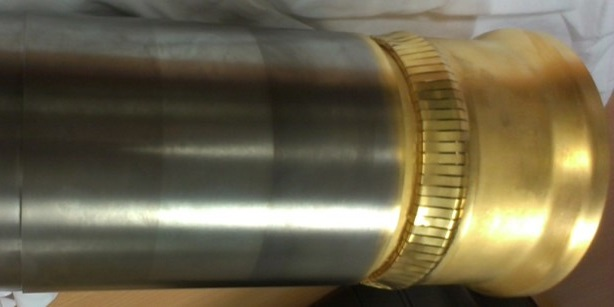
\includegraphics[width=1.0\linewidth]{figures/chap3/RF_contacts/RF_contact_CCFE_before.png}
	\caption{RF Contact prototype tested in 2014.}
	\label{fig:rfcontactccfebefore}
\end{marginfigure}

In a previous test campaign, a design proposed by the CYCLE consortium using brazed lamellae supported by a spring \sidecite{argouarch2014}, was tested in the T-resonator up to 1.7~kA during 1200~s but failed for larger current values due to a degradation of the contacts as illustrated in Figures\ref{fig:rfcontactccfebefore} and \ref{fig:rfcontactccfe}\sidecite{hillairet2015-1}. During previous tests on the T-resonator or in other testing devices, higher current densities have been reached when using commercial contacts such as Multi-Contact LA-CUT\sidecite{argouarch2013}. For this reason, the tests realized in 2014 were made using such kinds of commercial product. This T-resonator is described in next section and the tests made in 2014 are described in the following sections.

\begin{figure}
	\centering
	\includegraphics[width=1.0\linewidth]{figures/chap3/RF_contacts/RF_contact_CCFE}
	\caption{Result of the tests performed in 2014 with a prototype of RF contacts}
	\label{fig:rfcontactccfe}
\end{figure}

%\clearpage
% #####################################################
\subsection{The CEA/IRFM T-resonator}
CEA had setup a steady-state test bed, an actively water-cooled coaxial T-resonator illustrated in Figures~\ref{fig:rfcontacttresonatorillustration2} and \ref{fig:rfcontacttresonator2}, which allows testing coaxial components up to 45~kV and 2.25~kA in ITER relevant conditions of vacuum and temperature \sidecite{argouarch2013}. The setup consists in a rigid coaxial resonator, made of two main branches approximatively 2.2~meters long. Both branches are RF powered from a RF source feeding a T-junction and are ended by adjustable short-circuits referred as \textit{trolleys} hereafter. Such sliding short-circuits allow tuning the resonator matching configuration, in addition to the possibility to tune the RF frequency. A vacuum feed-through is located upstream of the T-junction, which allows the T-resonator to be vacuum pumped. Electric heating cables were inserted into both branches outer conductors for baking purposes. 

\begin{marginfigure}
	\centering
	\includegraphics[width=1.0\linewidth]{figures/chap3/RF_contacts/RF_contact_Tresonator2}
	\caption{Picture of the CEA/IRFM T-resonator.}
	\label{fig:rfcontacttresonator2}
\end{marginfigure}

\begin{figure}
	\centering
	\includegraphics[width=1.0\linewidth]{figures/chap3/RF_contacts/RF_contact_Tresonator_illustration2}
	\caption{Illustration of the CEA/IRFM T-resonator.}
	\label{fig:rfcontacttresonatorillustration2}
\end{figure}

All the inner and outer conductors of the resonator are actively water cooled by a cold water loop (4 bar/20\degC). The resonator, located in the TITAN facility, can also be connected to a hot water loop compatible with ITER specifications (up to 44~bar/250\degC). The water cooling temperature during RF operations in the ITER IC antenna is estimated to be 90\degC at the contact location. The DUT branch is optimized to maximize the current at the short-circuit. The current density at the outer conductor is approximatively half of the current density at the inner conductor (128/219=0.58). A similar setup is used on the opposite branch, with a reduced current at the short circuit due to the branch characteristic impedance configuration.

In order to match the resonator, both short circuit lengths can be tuned as well as the generator RF frequency, which allows a large operational flexibility. Voltage is measured in two locations of the resonator using voltage probes similar to the ones used in the JET and Tore Supra/WEST ICRH antennas \sidecite{helou2016}. The current at the short circuits is deduced from the measured voltages using a RF model of the resonator. To do this, both a lump\sidenote{The lump model is \href{https://github.com/jhillairet/tresonator}{available online}.} and a full-wave model in ANSYS HFSS and Designer have been created. These models parameters are the two short-circuit distances and the two equivalent resistances presented by each short circuits. Moreover, the material conductivities given in literature tables are given for bulk materials and are generally optimistic when dealing with surface coatings (Cf. the Section~\ref{sec:RF_windows} on the LHCD RF window R\&D). Thus, the Ohmic losses in the resonator model need also to be slightly increased to match reality, by a coefficient to be determined from the $Q$-factor measurement. In order to deduce all these quantities, first a low power measurement is performed on the matched resonator. The lump model short resistances and propagation losses are then optimized in order to match the measurements. 

An example of the result of the optimization is illustrated in Figure~\ref{fig:rfcontacttresonators11} where the transmission line model fits perfectly the measurements for equivalent resistances of 3.4 and 6.8~mΩ for the DUT and CEA short circuits respectively and additional propagation losses of +4.6\%. In this case, the resonator has been matched around 62~MHz. The choice of a frequency higher than the ITER bandwidth aims maximizing the RF losses and thus providing an additional engineering safety margin. 

\begin{figure}[h]
	\centering
	\includegraphics[width=1.0\linewidth]{figures/chap3/RF_contacts/RF_contact_Tresonator_S11}
	\caption{Resonator input voltage reflection coefficient ($S_{11}$) when matched at 62.64~MHz. The transmission line model of the resonator is fitted to the measurements in order to deduce the equivalent resistances of both shorts and line losses. }
	\label{fig:rfcontacttresonators11}
\end{figure}


Once the short circuit resistances are known, the model can determine the voltage and the current everywhere in the resonator for a given input power and short-circuit lengths. Figure~\ref{fig:rfcontacttresonatorcurrentvoltage} illustrates the voltage and current distribution for an input RF power of 60~kW. A maximum voltage of 40~kV is reached in the CEA branch while a maximum current of 2~kA is reached at the DUT short circuit. 

\begin{figure}[h]
	\centering
	\includegraphics[width=1.0\linewidth]{figures/chap3/RF_contacts/RF_contact_Tresonator_current_voltage}
	\caption{Voltage and currents inside the resonator for an input power of 60 kW at 62.64 MHz. L=0 indicates the location of the T-junction. Orange lines correspond to the DUT branch (L<0) and blue lines to the tuning (CEA) branch (L>0). Grey dashed vertical lines illustrate the locations of the voltage probes. The resonator characteristic impedances are illustrated in the third graph.}
	\label{fig:rfcontacttresonatorcurrentvoltage}
\end{figure}


%\clearpage

% ################################################
\subsection{Contact Materials}
\subsubsection{Base Materials}
Two types of base materials are relevant in the context of RF contact on ITER ICRH antenna: i) the contact louvers material (bulk) and ii) the base material of the facing conductor (Figure~\ref{fig:rfcontactmaterials}). For the facing conductors (or the contact holder), common materials are stainless steel and copper alloys. Stainless-steel has good mechanical strength and is a common material for manufacturing but its main drawback is its high electrical and thermal resistivity. In order to increase both the electrical and thermal conductivity, CuCrZr alloy is a good structural material commonly used in fusion engineering \sidecite{lipa2005, barabash2011}.

\begin{marginfigure}
	\centering
	\includegraphics[width=1.0\linewidth]{figures/chap3/RF_contacts/RF_contact_materials}
	\caption{Illustration of the contact materials.}
	\label{fig:rfcontactmaterials}
\end{marginfigure} 

\begin{marginfigure}
	\centering
	\includegraphics[width=0.5\linewidth]{figures/chap3/RF_contacts/RF_contact_creeping}
	\caption{Illustration of the creeping consequence.}
	\label{fig:rfcontactcreeping}
\end{marginfigure}

On the shelf LA-CUT louvers are made of either copper or copper-beryllium. However, copper is known to seriously creep in high temperature conditions (Figure~\ref{fig:rfcontactcreeping}), for instance during the thousands of hours of ITER baking phases at 250\degC. Since creeping would impact the contact pressure applied to the conductor and degrade the contact quality with time \sidecite{pauer2002}, pure copper louvers must be discarded. Copper-beryllium (CuBe), copper-nickel-beryllium (CuNiBe) and copper-chromium-zirconium (CuCrZr) alloys have lower creep rate as well as higher yield strength \sidecite{li2000, li2012}. The material properties of these alloys highly depends on their manufacturers and grades, but in a general way the yield strength of CuBe (>700~MPa) is higher than CuCrZr (around 450~MPa) and its thermal conductivity is lower (from 50 to 200 versus 320-340~\si{W/m.K}) \sidecite{li2012}. In addition, in a fusion reactor, high energy neutrons will produce Ni, Zn and smaller amount of Cobalt in copper and copper alloys, producing a significant decrease of the electrical and thermal conductivity  \sidecite{ garner1998, eichin2004}. At the contrary of CuCrZr, CuBe and CuNiBe contains Nickel (between 1.4 to 2.2\%) and Cobalt (between 0.30 to 0.60\%), which may induce higher intensity gamma-ray emitter 60Co after neutron irradiation. Depending of the total amount of these products, CuCrZr may be preferred to CuBe/CuNiBe in this context. Moreover, because of low fracture toughness and tensile elongations for temperatures higher than 250$\si{\degreeCelsius}$, CuNiBe appears to be not a suitable option unless improved thermo-mechanical treatment conditions are found \sidecite{zinkle2014}. For the latter reasons, the choice of a CuCrZr alloy for the contact louvers material has been made.

\subsubsection{Coating Materials}
Early current connector designs implementing metal-metal contacts were plagued with high friction, wear and heat generation mainly attributed to electrochemical oxidation and arcing \sidecite{Argibay2011, argibay2012}. For the electrical contacts working at high temperature and high vacuum, wear performance becomes critical and coatings can be used to improve their electrical performance and life-time. For RF applications, dozens of micrometers thicknesses are enough for contact materials, which is much lower than their required structural dimensions. Moreover, the geometry of the RF contact is usually complex and good uniformity of coating is required for the whole RF contact component. For these reasons, electroplating is generally used for RF contact coating.  

The ideal vacuum electrical contact coating materials should have the following specifications: high electrical conductivity, high thermal conductivity and good structural stability under high temperature, low friction coefficient and high wear resistance even under high temperature and high vacuum and if possible economic. It is difficult to find a material to meet all the above requirements, that are sometimes antagonistic. Compared with single electro-deposited metals, alloy deposition often provides superior properties. With certain composition ranges, the alloy electroplating layers can be harder, denser and have higher resistance to corrosion and wear. 

Silver is a well-used contact material, since it has the highest electrical and thermal conductivity of all metals (resistivity: 1.67~$\si{\micro \ohm cm}$) and is also resistant against oxidation. Electroplated silver is a worthy coating for temperatures less than 160$\si{\degreeCelsius}$ with good fretting performance and excellent electrical properties \sidecite{slade2014, talgner2014}. At temperatures higher than 100$\si{\degreeCelsius}$, recrystallization at temperature decreases the hardness to lower than 90~HV10, which can induce wear, cold welding and material migration. Coating thicknesses up to few tens of micrometers are generally deposited on the electrical contacts designed to withstand very high normal force (10-100~N), which is the case in this application. For these reasons, a thick silver-coating (>10$\si{\mu m}$) has been selected as a functional coating of the RF contact louvers.

\subsection{Sliding Tests}
\begin{marginfigure}
	\centering
	\includegraphics[width=1.0\linewidth]{figures/chap3/RF_contacts/RF_contact_LACUT_sliding_tests}
	\caption{Picture of the insertion and sliding test bed at CEA (Maestral, Pierrelatte)}
	\label{fig:rfcontactlacutslidingtests}
\end{marginfigure}

The contact prototype has been assembled into a static electromechanical load frame illustrated in Figure~\ref{fig:rfcontactlacutslidingtests}. The load frame was moved through an oven that can be baked to the required temperature, which is controlled with a precision of +/- 0.5$\si{\degreeCelsius}$. The force cell located on the top of the load frame is cooled by water and forced air to allow a stable temperature during the test. The sliding contacts (95 louvers) have been inserted in a steel holder (the male part) which can be inserted in a CuCrZr ring (the female counterpart). A diaphragm bellows is assembled between both parts and the assembly can be vacuum-pumped via a turbo-molecular pump. Centring brass elements were added to the setup in order to improve the coaxial alignment between male and female parts. The position accuracy of the male part is measured within +/- 0.5\% and the load is measured with a 5~kN force cell. 


The load frame was first used to measure the required insertion forces under atmosphere, then the sliding forces in an ITER relevant vacuum and 175$\si{\degreeCelsius}$ environment, which corresponds to an estimate of the operational temperature of the contacts. Up to 30 000 cycles with a 3~mm stroke were performed in vacuum at 175$\si{\degreeCelsius}$. The required insertion force up to approximatively 700~N for the first insertion and about 550~N the following insertions, which corresponds to 5.8~N per louver. When the contact is fully engaged, the sliding force is about 200~N (2.1~N per louver). After 10 cycles, a thin layer of silver is transferred from the louvers to the CuCrZr ring. 

Then, the test bed was pumped and baked to 175$\si{\degreeCelsius}$ with a brand new Multi-Contact band with 95 louvers assembled in the test bed. The measured pressure at 175$\si{\degreeCelsius}$ is $3.2\times 10^{-4}$~Pa. 5~000 cycles were made on an extension of 3~mm (1.5~mm back and 1.5~mm forth). The Figure~\ref{fig:rfcontactlacutslidingtestsresults} illustrates the load vs the cumulated distance travelled by the contact during these 5~000 cycles. It can be seen that the load is increasing then sharply decreasing over the cumulated distance of one meter, corresponding to the first 200-300 cycles. After one meter (>300 cycles), the load is almost constant and on the order of 250 N.


\begin{marginfigure}
	\centering
	\includegraphics[width=1.0\linewidth]{figures/chap3/RF_contacts/RF_contact_LACUT_sliding_tests_results_15000}
	\caption{Close-up picture of some louvers after 5 000 and 15 000 sliding strokes. The CuCrZr louvers are little damaged. The silver coating has been removed from the louver's tip. Results are similar after 30 000 cycles.}
	\label{fig:rfcontactlacutslidingtestsresults15000}
\end{marginfigure}

After 5 000 cycles, the test bed was opened and inspected. The silver coating of the contact is totally removed at the tip of the louvers (Figure~\ref{fig:rfcontactlacutslidingtestsresults15000}). Clear scratches are visible on the CuCrZr ring, and a detailed observation of the contact shows the removal of the silver layer on the tip of louver. The area of contact (1800x900µm) after 5 000 cycles is flattened and the CuCrZr base is clearly visible. From the curves of the Figure~\ref{fig:rfcontactlacutslidingtestsresults}, three sliding regimes can be identified. During the first tens of cycles, the sliding force magnitude increases. This increase is attributed to the machining of the silver (on the louvers) and the CuCrZr (on the ring), where the softer silver forms an interfacial layer (‘buttering’). Once the silver coating fully removed in the sliding track, the abrasion of the louver tip leads to a smaller compression (by consequence the LA-CUT stainless-steel elastic skeleton is less constrained) which tends to decrease the contact force. At a certain point, an established regime is achieved (CuCrZr louvers vs CuCrZr ring).  

Subsequent series of 10 000 and 15 000 cycles were made with the same contact band up to a total of 30 000 cycles (90 meters), corresponding to the required operational life of the ICRH antenna in ITER. For each series, the mechanical position of the contact stabilized in a few cycles and then the average load remained almost constant to 250 and 300~N during the remainder of the cycles. The wear on the louvers after 30~000 cycles is of the order of 150~µm (Figure\ref{fig:rfcontactlacutlouvertip}, top picture). The wear of the CuCrZr ring after 30 000 cycles (90 meters) is of the order of 60-80 µm on a width of 0.1~mm (Figure\ref{fig:rfcontactlacutlouvertip}, bottom picture). The remaining question of the impact of such scratches on the RF current flow has not been investigated and could be investigated by performing RF tests with the damaged contacts.


\begin{marginfigure}
	\centering
	\includegraphics[width=1.0\linewidth]{figures/chap3/RF_contacts/RF_contact_LACUT_louvertip}\\
	\includegraphics[width=1.0\linewidth]{figures/chap3/RF_contacts/RF_contact_LACUT_scratches}
	\caption{Top: zoom on the tip of louver after 30 000 cycles. The wearing of the louver is of the order of 150 µm. Bottom: Picture of the CuCrZr ring after 30 000 cycles. The 1.5 mm long scratches depth (in the middle of the picture) is of the order of 60-80 µm on a width of 0.1 mm.}
	\label{fig:rfcontactlacutlouvertip}
\end{marginfigure}


\begin{figure*}
	\centering
	\includegraphics[width=1.0\linewidth]{figures/chap3/RF_contacts/RF_contact_LACUT_sliding_tests_results}
	\caption{Average Sliding Load versus the equivalent distance travelled by contact band.}
	\label{fig:rfcontactlacutslidingtestsresults}
\end{figure*}

The main outcome of these sliding tests is the rapid wearing of the thick silver coating. The 30~µm thick silver-coating made on the LA-CUT louvers is removed during approximately a hundred of stroke cycles made at 175\degC under vacuum, which represents a cumulated distance travelled lower than one meter. Once this layer removed, we end up with a friction between the CuCrZr of the louver and the material facing the louver, the CuCrZr of the ring in this case. 

\subsection{RF Tests}
A new qualification campaign has been setup in 2015-2016 in order to test a new Multi-Contact LA-CUT prototype made of 30~µm silver coated CuCrZr louvers (Figure~\ref{fig:rfcontactlacuttest}). This prototype has also been assembled into the RF resonator in order to test it under ITER relevant conditions. 

\begin{figure*}
	\centering
	\includegraphics[width=1.0\linewidth]{figures/chap3/RF_contacts/RF_contact_LACUT_test}
	\caption{LA-CUT setup before assembly into the RF resonator}
	\label{fig:rfcontactlacuttest}
\end{figure*}

In order to reproduce the ITER conditions, the Device-Under-Test (DUT) is assembled on a copper coated stainless-steel holder, ending the inner conductor of the DUT branch. Both this inner conductor extension and the trolley have been connected to the hot water cooling loop, tuned to a 90\degC inlet temperature. Prior to RF tests, the resonator has been pumped and baked up to 120\degC for 20 days. After baking, the pressure was $8\times10^{-6}$~Pa. During RF tests, the resonator was water cooled at 20-25\degC while the DUT was water cooled at 90\degC to mimic ITER operations. RF conditioning shots consisting in kilowatt range of power pulses were performed for a set of various frequencies around the match frequency, in order to sweep the voltage and current node locations in the resonator. 

Once conditioning pulses do not reflect power at the match frequency, the input power has been progressively increased for short durations. Within 90 shots, the target current specification of 2.25~kA has been reached for 100~ms, then up to 5~s by increasing duration steps. The current was progressively increased in both amplitude and shot duration. During RF shot, the pressure was monitored for outgassing, but this time we allowed larger increases of the pressure, keeping an automatic safety interlock ($2\times10^{-2}$~Pa). It was found that the pressure increased after few tens of seconds, sometimes up to $10^{-2}$~Pa, but then stabilized and then decreased during the RF shot. Thus, the current was increased to 1.2~kA over up to 1200~s without pressure increase larger than the safety interlock. Light emission was continuously monitored during these shots, starting after 60 to 120~s depending on the shot. Moreover, it was observed that the light emission changed both in brightness (increase or decrease) and locations during the shot duration as illustrated in Figure~\ref{fig:rfcontactlacutlightemission}.

\begin{figure}[h]
	\centering
	\includegraphics[width=0.7\linewidth]{figures/chap3/RF_contacts/RF_contact_LACUT_light_emission}
	\caption{Webcam snapshots during shot \#3379 (1.2kA/1200s).}
	\label{fig:rfcontactlacutlightemission}
\end{figure}

At this point and for higher RF power, it was observed that the number of arc events detected (from reflected power) increased, sometimes led to the complete un-matching of the resonator, often at the beginning of the pulse but even after hundreds of seconds of RF power. In order to reduce these effects, the input power was then ramped up instead of applying the full power from the beginning of the RF pulse. Using this strategy, the current has been increased up to 1.9~kA during 300~s. After this last pulse, outgassing increased up to $8\times 10^{-2}$~Pa during the cool down of the DUT and the resonator was detuned. Outgassing was severe for the following shots and it was not possible to continue RF tests. The inspection of the DUT side of the resonator showed that the DUT contact louvers were burnt and melted in various places, and burn/arc traces were also observed on the trolley contact louvers (Figure~\ref{fig:rfcontactlacutmelt}). 


\begin{figure}[h]
	\centering
	\includegraphics[width=1.0\linewidth]{figures/chap3/RF_contacts/RF_contact_LACUT_melt}
	\caption{Pictures of the RF contacts after failure. Left picture: inner conductor DUT contact holder. Right picture: outer conductor contacts on sliding trolley.}
	\label{fig:rfcontactlacutmelt}
\end{figure}

The target performance, i.e. a peak current of 2.25~kA at 62~MHz, has been reached only on short pulse durations (below 10~s). Currents between 1.2~kA and 1.3~kA have been reached in steady-state conditions (with duration higher than 60~s up to 1200~s) without any problem monitored on RF or pressure sensors. An inspection of the contacts has been performed after having reached currents lower than 1.3~kA and do not show any visual damage. The RF current has been increased up to a maximum of 1.9~kA during 300~s, but it was not possible to increase the current to larger values. The targeted steady-state RF tests specifications on the contact have not been achieved, due to the failure of the contacts at lower current values (1.9~kA). 

From RF and thermal modelling of the contact, the following failure mechanism is proposed. Because of its relatively low electrical conductivity, high RF losses are deposited at the surface of the contact steel spring elements. Since the heat accumulated in this steel part is poorly evacuated in the present design, its temperature increases which reduces its stiffness. As the contact force between the louvers and the fix part decreases accordingly, the contact resistance at the louver tips increases, leading to a vicious circle increasing the heat flux on the louvers up to melt some CuCrZr louvers. As the number of louvers in contact with the fix part decreases, the current is diverted to the remaining louvers, thus increasing again the heat fluxes and finally lead to the failure of all louvers in cascade. 



\subsection{Failure Mechanisms and Material R\&D}
Even though significant progress about the mechanical design of RF sliding contacts and the necessary knowledge about their material had been achieved in the previous R\&D phases, there is still a large gap between the obtained results and the ITER RF sliding contact design specifications. The development of an ITER RF sliding contact is the combination of mechanical structure design and material selection. The previous studies mainly focused on the RF current carrying capability of the LA-CUT commercial product. However, the failure mechanism of the RF contact was not deeply researched. As a result, the main parameters or factors that can affect the RF contact's stability were not clearly understood. In the PhD thesis of Zhaoxi Chen\sidecite{chen2018}, the failure mechanisms of the LA-CUT commercial electrical contact under ITER ICRH application conditions have been deeply investigated and relationship between the LA-CUT operational performance with the material selection has been analyzed. Direction to the material selection for the ITER ICRH RF sliding contact development have also been given. 

\begin{marginfigure}
	\centering
	\includegraphics[width=1.0\linewidth]{figures/chap3/RF_contacts/RF_contact_Rc}
	\caption{The contact resistance between two metal of respective resistivity $\rho_1$ and $\rho_2$ is defined by $$R_c=\frac{\rho_1+\rho_2}{4a}$$ where $a$ is the average radius of the metal-to-metal contact area \citeauthyear{holm2011}.}
	\label{fig:rfcontactrc}
\end{marginfigure}

From FEM models and by performing electrical-thermal and thermal-hydraulic analyses, Zhaoxi Chen analysed the failure mechanisms of ITER RF sliding contacts based on a prototype of the Multi-Contact LA-CUT product \sidecite{chen2017-2}. Using the results of the test campaign described in previous sections, it was found that the steady-state operating temperature of the RF contact louver linearly increases with the contact resistance ($R_{contact}$) increase (Figure~\ref{fig:rfcontactrc}). In order to maintain the temperature of the RF contact louver below 250\degC, it has been calculated that the $R_{contact}$ should be lower than 6.5~$\si{\milli\ohm}$/louver. This parameter drives the choice of the materials to be used to reduce the operational contact louver temperature. If the RF conductor is made of 316L stainless steel, increasing cooling parameters (such as mass flow rate and velocity) has almost no effect to improve the cooling performance of the contact louver. Actively cooled CuCrZr is strongly suggested as base material of the RF contacts support. 

During his PhD, Zhaoxi Chen developped a multi-functional tribometer \sidecite{chen2017-3} which can mimic ITER-relevant vacuum and temperature conditions for material evaluation for the ITER RF sliding contact (Figure~\ref{fig:rfcontacttribometerzhaoxi}). Although some commercial vacuum tribometers which could even measure contact resistances exist, no tribometer were found having in addition a sample heating capability. Moreover, any commercial vacuum tribometer needs to be opened to adjust the normal contact force, which is time-consuming and not compatible with the time allowed for the material study in this thesis, as we needed to adjust the normal contact force frequently. Thus, a multi-functional tribometer which can mimic the ITER environment conditions and be operated conveniently and reliably was developed. This tribometer has been used to characterize the friction and contact resistance properties of various samples of materials. A French innovation patent concerning the loading system has been submitted and authorized\sidecite{chen2017-4}.   

\begin{figure}[h]
	\centering
	\includegraphics[width=1.0\linewidth]{figures/chap3/RF_contacts/RF_contact_tribometer_zhaoxi}
	\caption{Illustration of the vacuum tribometer develloped in the frame of the PhD thesis of Zhaoxi Chen \citeauthyear{chen2018}}
	\label{fig:rfcontacttribometerzhaoxi}
\end{figure}

The feasibility of applying Au-Ni, Ag, Ag-Sb and Rh as functional coatings for ITER RF sliding contacts have been evaluated from material characterizations and the tribometer developped (Figure~\ref{fig:rfcontacttribometerresults}) \sidecite{chen2017-2, chen2018}. The base material of the RF contact louvers was selected as CuCrZr. The supporting conductor can be made of 316L or CuCrZr. From FEM analyses, the $R_{contact}$ of one louver should be lower than 6.5~$\si{\milli\ohm}$. In order to improve the electrical and tribological performances of the sliding contact, the application of functional coatings have been found to be mandatory. From the commonly used material in the electrical industry, the specific ITER environment conditions of vacuum and temperature lead to the choice of Au-Ni, Ag, Ag-Sb and Rh coatings. 

\begin{figure}[h]
	\centering
	\includegraphics[width=1.0\linewidth]{figures/chap3/RF_contacts/RF_contact_tribometer}
	\caption{Example of measurement of contact resistance $R_{contact}$ in vacuum conditions in the tribometer. }
	\label{fig:rfcontacttribometerresults}
\end{figure}

In addition, the development of Au-Ni/a-C and Au-Co/WS2 composite coatings and their application as electrical functional coatings in ITER has been investigated \sidecite{chen2020}. Although Au-Ni and Au-Co are commonly used coatings on electrical and electronic industries, their composite coatings were not deeply considered in the fusion research field. As seen with sliding tests, ITER ICRH RF sliding contacts will face severe adhesive wear during operation and applying solid lubricants on them is very promising. Satisfactory Au-Ni/a-C composite coatings were deposited by magnetron sputtering. A significant hardness improvement has been demonstrated in comparison with Au-Ni coating. However, due to the low lubricating efficiency of carbon materials in vacuum, these composite coatings do not have advantages in minimizing friction coefficient and wear rate compared with Au-Ni coating. Finally, an Au-Co/WS2 electroplating composite coatings process has been developed and used. A technical breakthrough was made in the WS2 particle dispersion in aqueous cyanide electrolyte\sidecite{chen2020}. Their high efficiency in minimizing friction and wear rate under ITER conditions were proved. 

Before this thesis, no systematic study and evaluation of common functional coatings under ITER relevant conditions have been made. During this thesis, the above functional coatings were electro-deposited on CuCrZr and 316L substrates and they were deeply characterized regarding their diffusion phenomena with their substrates or with another coating after 250\degC thermal aging process. In addition, thermal aging effects on the coatings'morphology, hardness, adhesion performance, crystal structure, electrical and tribological performances were evaluated. The coefficient of friction and contact resistance $R_{contact}$ values have also been measured. All these results provide a good reference for the future studies of ITER RF sliding contacts or other projects.


\subsection{Summary of this section}

Radio-Frequency tests have been performed at CEA/IRFM using a RF resonator equipped with Multi-Contact LA-CUT/0.25/0 prototype, whose louvers are made in CuCrZr with a 32~µm thick silver coating. From ITER IC antenna specifications, the targeted test specifications were a peak current of 2.25~kA during 20~minutes (1200~s), under vacuum pressure below $10^{-3}$~Pa and a water cooling temperature of 90\degC $\pm$ 5\degC at a RF frequency of 62~MHz. The required current performance has been reached on durations inferior to 60~s. Currents between 1.2~kA and 1.3~kA have been reached in steady-state conditions, for durations larger than 60~s and up to 1200~s, without any problem monitored on RF or pressure sensors, despite monitoring light emission. The RF current has been increased up to a maximum of 1.9~kA during 300~s, but it was not possible to increase the current to larger values. The targeted steady-state RF tests specifications on the contact have not been achieved, due to the failure of the contacts for which both the CuCrZr louvers and the steel holder of the contact band melted in various locations. 

Sliding tests have shown that the coating located at the tip of the louver barely survives to more than hundreds of sliding cycles, the reason of existence these coatings could be challenged in regard of the number of the sliding cycles expected in the antenna. However, one should keep in mind that since most of the louver coating is not damaged during sliding, the gain in heat losses reduction is still important. Moreover, the Ag coating protects the CuCrZr substrate from corrosion. A remaining question is the impact of the louver tips silver-coating removal and of the generated scratches on the ring surface on the RF performances. This point could be investigated by performing RF tests with damaged contacts. Finally, in order to increase the life time of the louver coating, advanced coating made of silver or gold alloys with increased hardness could be investigated.

A dedicated PhD oriented on material science has been setup with the Toulouse University in order to analyse the failure mechanisms of these RF contacts\sidecite{chen2018}. During this thesis, a vacuum tribometer has been designed and used to measure the material characteristic in vacuum environment. In combination to FEM analysis, the conclusions of this work are that material selection is the main driver of the both RF and thermal performances of these RF contacts, in particular when used under vacuum environment. The bulk and coating materials must selected in order to optimize mechanical and RF performances. From this analysis, a new set of test with improved RF contacts and choice of coatings and bulk materials will be made at CEA/IRFM in 2021.



\section{Perspectives}
While the Ion Cyclotron Resonance Heating have been proved working effectively to heat the core plasma of various fusion  experiments, the method has also several drawbacks. 

As current ICRH antennas radiates  wave  components with $k_\parallel > k_0$, these waves are evanescent from the antenna up to the fast wave cut-off electron density, located few centimetres away in front of antenna. As this distance increases, the coupling efficiency of an antenna decreases, which often leads to operation issues. In future machine such as ITER or the future European fusion reactor DEMO, the distance from the antenna to the plasma will become even larger.

In addition, transmitting the maximum amount of RF power while protecting the RF sources from reflected power requires matching system(s). A consequence of these matching unit(s) is that the voltages and currents in the antennas can reach very high values and jeopardize the operation safety when exceeding the voltage stand-off limits.

Hence, instead of resonant antennas, Travelling Wave Arrays (TWA) antennas would be a good candidate to perform ICRH in tokamaks since they solve these both drawbacks. Having a lower power density in comparison to resonant antennas, TWA antennas have hence lower voltages, avoiding exceeding voltage stand-off \sidecite{messiaen2017, ragona2017-1}. In addition, as the number of radiating elements is larger than in conventional antennas, the radiated spectrum is narrower which enhances antenna coupling to the plasma, hence allowing coupling RF power from larger distances to the plasma than current antennas. The main drawback is TWA antennas require a larger toroidal space to fit a higher number of straps. However, since the antenna does not require fancy power dividers and matching units, the volume required behind the radiating elements only consist in the feeding transmission lines. In the context of fusion reactor, this reduced footprint is a very interesting advantage when dealing with neutron-induced activation and heat losses but also leaves more space for lithium breeding blankets. For these reasons, TWA antenna designs have been proposed for DEMO \sidecite{ragona2016, ragona2019-1, noterdaeme2019}. 

Despite not being a new concept \sidecite{moeller1994, vdovin2009} and already been tested at moderate powers \sidecite{ikezi1997, ogawa2001}, TWA antennas have so far never been tested for Ion Cyclotron minority heating at relevant powers. This is why, in the frame of the collaboration between LPP Brussels and ASIPP laboratories, a conceptual TWA antenna for WEST has been made designed \sidecite{ragona2019}. This concept is illustrated in Figure~\ref{fig:twawest}. As an intermediate step between the concept and a final WEST antenna, a high power mock-up has been manufactured and should be tested under vacuum in the TITAN test bed at IRFM in 2021. Depending on the results of this test, a WEST TWA antenna could be expected in the next years in order to demonstrate the theoretical benefits of such antenna over classic resonant structures.

\begin{marginfigure}
	\centering
	
	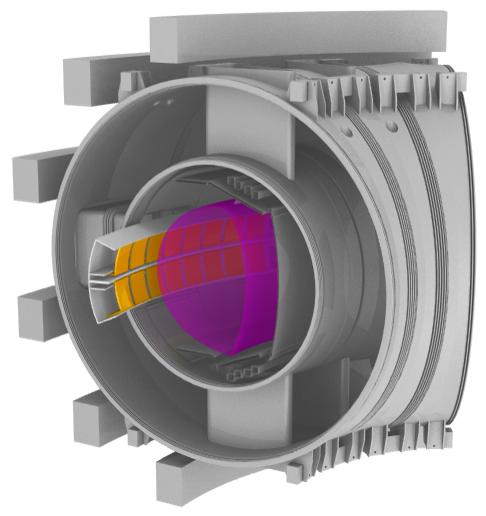
\includegraphics[width=1.0\linewidth]{figures/chap3/TWA/TWA_WEST}
	\caption{Conceptual illustration of a possible configuration of a WEST Traveling Wave Array antenna (Image Credit R.Ragona).}
	\label{fig:twawest}
\end{marginfigure}



\section{Chapter Summary}
In this chapter we first gave the necessary theoretical background to address the design of high-power Ion Cyclotron Resonance Heating systems. 

In the frame of the upgrade of the Tore Supra tokamak to WEST, the RF design of the WEST ICRH antenna has been performed. The antenna coupling has been improved using the COMSOL software. Other elements of the antenna have been optimized to leave more space for water cooling, making the WEST ICRH antennas the first load-resilient ICRH antennas compatible with CW operation.

The complete RF model of the WEST ICRH antennas has been modelled using the open-source Python package \href{http://scikit-rf.org/}{\texttt{scikit-rf}}, which the author is maintainer. The WEST ICRH antenna is modelled by connecting the various elements that compose it, separately full-wave modelled from final CAD models. Tunable elements, such as the matching capacitors, can be either created from ideal lump components or from interpolating full-wave calculations performed at various capacitance configurations. Being open-source, using \texttt{scikit-rf} to create the antenna numerical model with reproducible work-flow adds confidence in the fact that future users could use/maintain and extend it.

The three WEST ICRH antennas have been commissioned and used on WEST plasma between 2017 and 2019. The commissioning phase was relatively short, of about two days for each antenna to reach 1 to 1.5~MW. In the C4 campaign, after this commissioning phase, all three antennas have been operated simultaneously on WEST plasmas, leading to 5.8~MW coupled ICRH power after around 50~plasma discharges (close to 2~MW per antenna). While these results are very encouraging, some work remains for the future WEST campaigns to achieve reliably the target performances of 9MW/30s or 3MW/1000s.

In parallel, Radio-Frequency tests have been performed at CEA/IRFM using a RF resonator equipped with RF contact prototypes. It is planned to use these contacts inside the ITER ICRH antennas and these tests aimed to verify their compatibility with the ITER specifications. However, while the required current performances has been reached on durations inferior to 60~s and half-current target reached in steady-state conditions, these contacts failed for higher current levels and longer durations. A dedicated PhD oriented on material science has been setup in order to analyse the failure mechanisms of these RF contacts. The conclusions of this work are that material selection is the main driver of the both RF and thermal performances of these RF contacts, in particular when used under vacuum environment. Following the recommendations made by this work, a new set of test with improved RF contacts and choice of coatings and bulk materials will be made at CEA/IRFM in 2021.


%TWA \sidecite{ragona2019-1, melnikov2020} TWA WEST \sidecite{ragona2019}
